
\begin{center}
{\Large\bfseries \PaperTitle\par}
\vspace{12pt}
\AuthorNames\par
\vspace{5pt}
\AuthorAffiliations\par
\vspace{5pt}
\Correspondence\par
\end{center}
\vspace{8pt}
\section*{Abstract}
The cost of spatial transcriptomics motivates reconstruction of molecular profiles from sparsely measured tissue locations. We introduce GraphPathology, a geometry-aware framework that separates graph representation learning of histological context from molecular reconstruction using sparse observed anchors. Development comparisons use coordinate-defined tissue graphs to contextualize image features; an observation-dependent graph connects unmeasured locations to available molecular anchors. This formulation makes spatial support and information access explicit across image, molecular and fusion predictors. We evaluated a predefined 50-gene panel in 25 held-out patients from two independent breast cancer studies. At 20\% distributed coverage, molecular reconstruction achieved median patient Pearson correlations of 0.359 and 0.416, compared with 0.059 and 0.075 for image-only prediction. In the 22-patient replication, increasing coverage from 10\% to 40\% improved correlation and reduced error in every patient. Contiguous regional completion remained harder, and fixed image fusion provided no reproducible external gain. Reconstruction using one fifth of locations motivates a potential fivefold reduction in location-dependent measurement costs under proportional costing, but total assay savings require prospective validation. Code: \url{\CodeRepository}.

\noindent\textbf{Keywords:} spatial transcriptomics; sparse reconstruction; geometry-aware graph learning; spatial transcriptomics imputation; histopathology; breast cancer

\linenumbers
\section{Introduction}
Spatial transcriptomics (ST) retains anatomical context while measuring gene expression across heterogeneous tissue\cite{stahl2016}. However, dense profiling can be expensive, and many acquisition designs provide expression at only a subset of the tissue locations. Histology is comparatively available, motivating methods that leverage both tissue morphology and the geometry of measured molecular profiles\cite{jaume2024,he2020}. A computational approach to reconstructing unmeasured locations could support more efficient study designs, but the prediction task and the measured information available at inference must be specified explicitly.

In breast cancer, spatially resolved molecular measurements have revealed tissue-architecture features that are difficult to characterize through bulk assays\cite{andersson2021,wu2021,bassiouni2023}. We consider a precise reconstruction task: gene expression for a prespecified panel is observed at a subset of retained locations within one tissue section, and the goal is to estimate that same panel at remaining locations. This differs from inferring an entirely unassayed panel or predicting expression from histology alone. Histological appearance and physical coordinates are known for all retained locations, but observed expression vectors are restricted to the measured anchors.

\subsection{Related work}
Histology-to-ST prediction has progressed from local convolutional approaches such as ST-Net\cite{he2020} and DeepSpaCE\cite{monjo2022} to combined visual-context models. Hist2ST uses Transformer and graph components\cite{hist2st2022}, THItoGene studies richer histology representations\cite{thitogene2024}, and FmH2ST uses feature-informed links between potentially distant histological regions\cite{fmh2st2025}. These methods demonstrate that graph-based context and long-range histological associations are established approaches; neither idea in isolation is a novelty claim for GraphPathology. CMRCNet\cite{liu2026} and cross-cohort benchmarking\cite{wang2025} further motivate careful claims about transportability.

A complementary line of work conditions reconstruction on experimentally observed spatial expression. XFuse combines molecular measurements and images for super-resolution inference\cite{bergenstrahle2022}; TESLA combines spatial and visual data to map tumors at high resolution\cite{tesla2023}; and iStar integrates ST with high-resolution histology\cite{istar2024}. More recent approaches target sparse-measurement and efficient-acquisition settings: Sparser2Sparse learns from sparsely sampled sections\cite{sparser2026}, SCR$^2$-ST considers adaptive sampling\cite{scr2st2026}, and PanoSpace addresses continuous tissue-wide reconstruction with additional modalities\cite{panospace2026}. Spatial graph methods such as SPACEL address related spatial-domain and multi-section tasks\cite{spacel2023}. These methods differ in required modalities, acquisition assumptions, target resolution and training strategy. We do not claim that interpolation, sparse acquisition, graph neural networks, or joint image--molecular inference originated in this work; direct head-to-head performance comparisons with these published systems were not conducted.

\subsection{Methodological contribution and study objectives}
We formulate \emph{GraphPathology} as a geometry-aware and observation-constrained reconstruction framework with two distinct spatial pathways. First, a tissue-context graph constructed from physical coordinates determines the neighboring image embeddings that inform a contextual expression representation. We compare fixed mean-pooling, GCN\cite{kipf2017} and GraphSAGE\cite{hamilton2017} aggregation within a controlled architecture, including spatial-topology controls. Second, at prediction time a molecular-support graph links an unmeasured site to its available measured anchors, enabling observed gene expression to enter predictions without revealing the hidden target labels. These are different graphs: one contextualizes morphology; the other transports \emph{measured} molecular information.

The molecular-support graph is defined from the observed set and physical distance, without a hard spatial-distance cutoff. It can therefore connect locations across substantial gaps where no measured molecular neighbors are nearby, although reliability may decrease with distance. The contextual image GNN instead uses a single local aggregation step; we do not claim that it learned global dependencies or that it drove the final external improvements. The most consequential external results are from sparse molecular reconstruction under distributed and contiguous-missing-region protocols, compared with a frozen image predictor and calibrated fusion.

We test three central questions: (i) the gain available from observed molecular anchors at restricted measurement budgets, (ii) how distributed and contiguous absence differ at the protocol level, and (iii) whether the frozen image branch provides incremental predictive value after the anchors are supplied. We evaluate these questions in two independent breast-cancer studies, preserving patient-level analyses, fixed gene panels and the original negative controls. A 20\% measurement budget represents fivefold fewer profiled locations, but does not itself demonstrate fivefold savings in total experimental costs.

\section{Results}
\subsection{A staged evaluation separated development from fresh replication}
The analytical design distinguished dataset roles before interpreting performance (Fig.~\ref{fig:overview}; Table~\ref{tab:cohorts}). The development cohort contained 35,536 paired locations from four HEST invasive ductal carcinoma patients, with two patients used for training, one for validation and one for the primary development evaluation. HER2ST contributed eight patients and 3,455 locations to an initial transportability test and was subsequently reused for calibration development; it was therefore not treated as an untouched final validation cohort. The Wu study contributed six patients, of whom three were reserved for evaluation after the other three were used to establish a frozen calibration object. The second replication used the first numbered section from each of 22 Bassiouni patients, selected from source metadata before outcome evaluation. All 30,003 locations from these selected sections were assigned to evaluation, with no Bassiouni-specific training, calibration or method selection.

Fresh replication thus comprised 25 evaluation patients across two independent studies, totaling 38,484 retained locations. Both studies contained all 50 primary genes in their original order. HER2ST analyses used a 40-gene intersection and were not pooled with 50-gene summaries. The public external histology inputs were substantially downsampled: the nominal 112-\um{} image patch contained only 15 or 25 native pixels in the Wu cohort and 24--29 native pixels in the Bassiouni cohort. Consequently, these datasets provide direct evidence about molecular interpolation, but only a resolution-limited test of the frozen histology predictor.

\begin{figure}[!htbp]
\centering
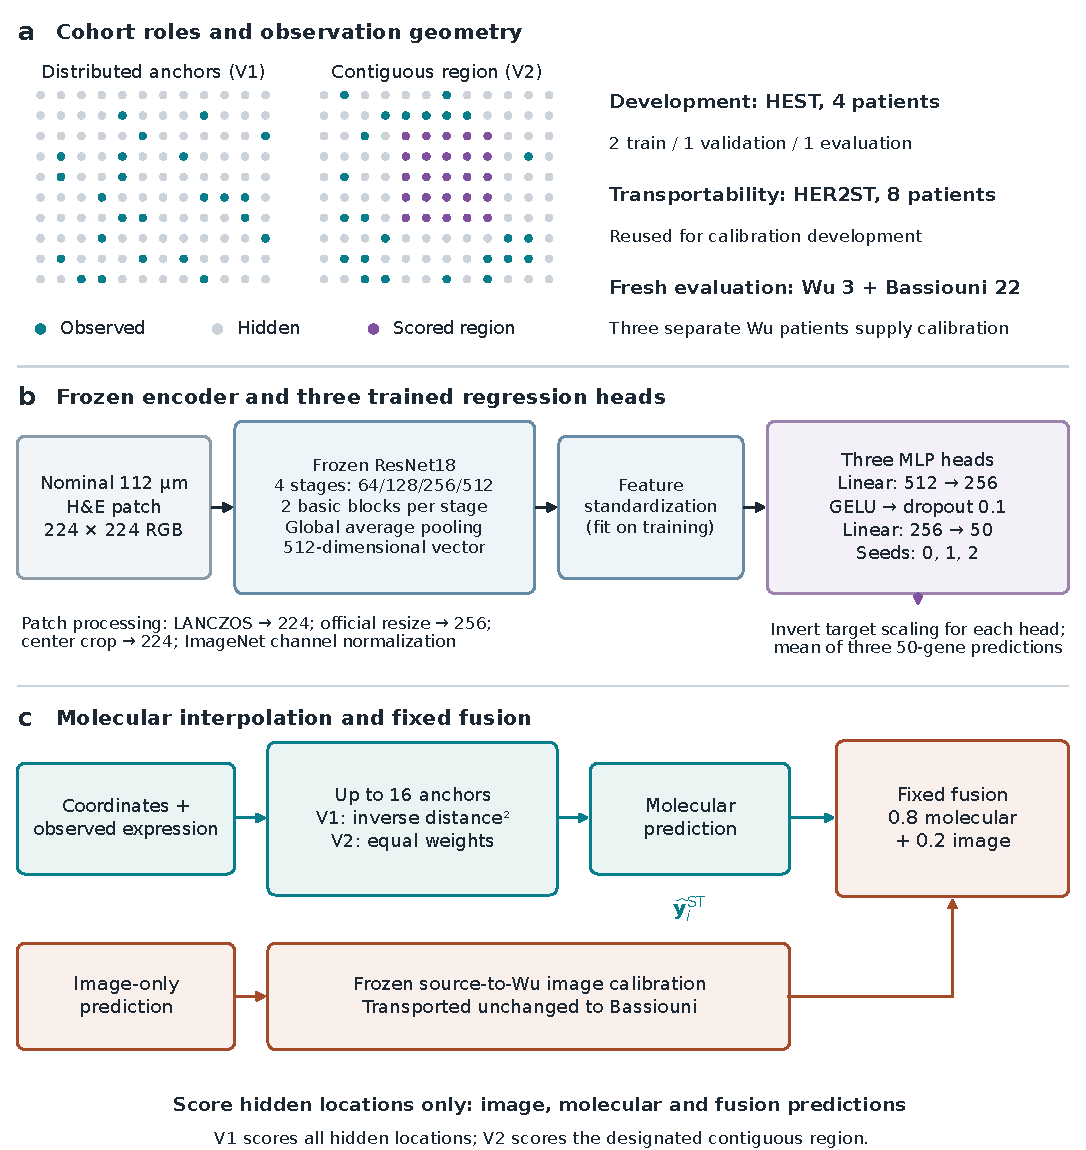
\includegraphics[width=\textwidth,height=0.72\textheight,keepaspectratio]{figures/Figure1.pdf}
\caption{\textbf{Study design and neural-image/molecular reconstruction architecture.} \textbf{a,} Cohort roles and illustrative observation geometries. Teal locations are observed molecular anchors; gray locations are hidden; purple locations form the contiguous scored region. The synthetic spatial examples illustrate 20\% coverage and are not patient measurements. The Wu calibration and evaluation groups contain different patients. \textbf{b,} The frozen ImageNet ResNet18 maps histology to a 512-dimensional vector after global average pooling; the ImageNet classifier is removed. External nominal 112-\um{} patches are first resized to $224\times224$ with LANCZOS, then processed by the official resize-to-256, central-crop-to-224 and channel-normalization transform. Feature scaling fitted on the training patients precedes each $512\rightarrow256\rightarrow50$ MLP, with GELU activation and dropout 0.1 after the hidden linear layer. The three heads use seeds 0, 1 and 2. Their predictions are inverse-scaled to the common target units and averaged. \textbf{c,} Molecular interpolation uses up to 16 observed neighbors, with inverse-distance-squared weighting for distributed evaluation (V1) and equal weighting for contiguous regional completion (V2). Fixed fusion combines this output with the calibrated image prediction using weights 0.8 and 0.2. The uncalibrated image ensemble is also evaluated separately. Calibration uses the development-training and Wu calibration patients and is transported unchanged to Bassiouni. Evaluation uses hidden locations only. V1 and V2 differ in weighting and scoring support as well as observation geometry.}
\label{fig:overview}
\end{figure}

\begin{figure}[!htbp]
\centering
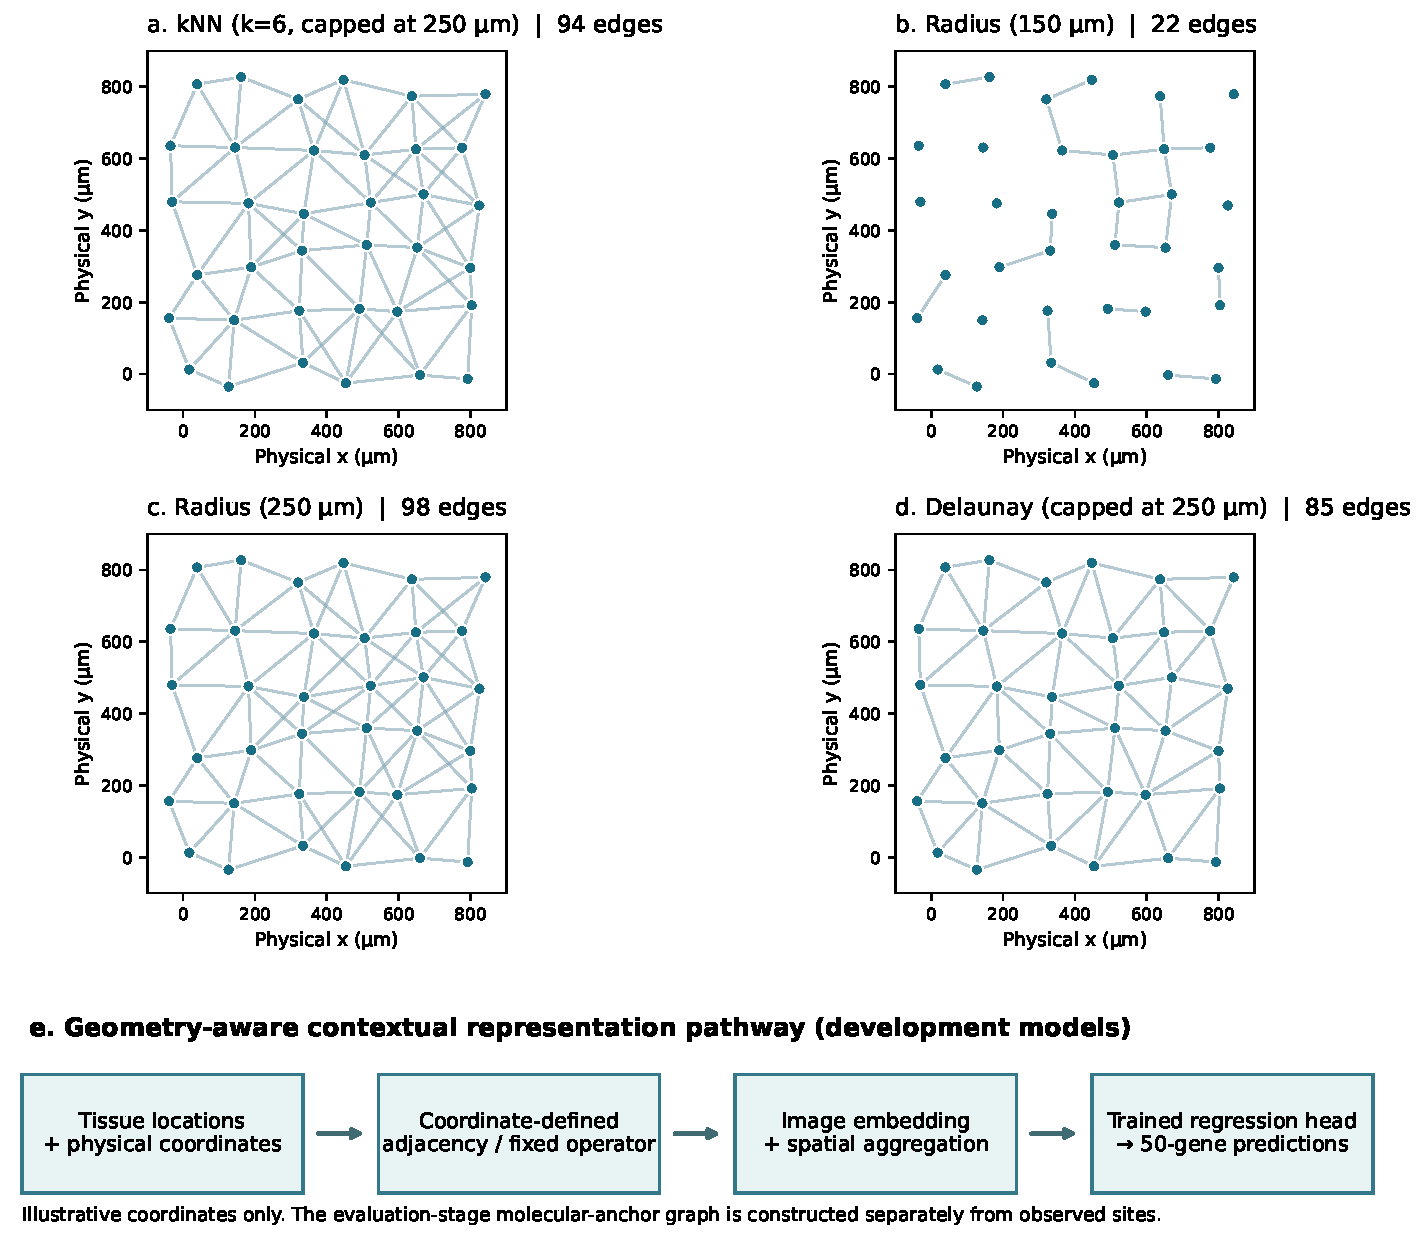
\includegraphics[width=\textwidth,height=0.78\textheight,keepaspectratio]{figures/Figure2.pdf}
\caption{\textbf{Geometry-aware graph construction and contextual representations.} \textbf{a--d,} The same 36 synthetic tissue locations are connected by (a) a symmetrized six-nearest-neighbor graph with a 250-\um{} distance cap, (b,c) 150- and 250-\um{} radius neighborhoods, or (d) a 250-\um{}-capped Delaunay graph. Coordinates and axes are identical across panels and all retained edges are displayed. Symmetrization means that a node can have more than six neighbors. \textbf{e,} Geometry determines a fixed adjacency/aggregation operator acting on the frozen image embeddings before an expression-regression head. The molecular-reconstruction stage uses a separate observation-dependent graph joining hidden locations to up to 16 measured molecular anchors. Synthetic points illustrate the architecture only, not a fitted patient graph or a performance result.}
\label{fig:graph_architecture}
\end{figure}
\begin{table}[!htbp]
\caption{\textbf{Cohorts and their analytical roles.} Counts refer to retained locations and patient-level study roles, not independent spot replicates. The same eight HER2ST patients were first inspected for transportability and subsequently used for calibration development. The Wu study contains 15,601 locations in all six patients; only 8,481 locations from its three evaluation patients enter fresh validation. All 22 Bassiouni patients were evaluated without new training or calibration. ``Pixels per patch'' refers to the native image information in a nominal 112-\um{} field of view, before resizing. The primary panel was fixed in development.}
\label{tab:cohorts}
\centering\small
\begin{tabularx}{\textwidth}{@{}>{\RaggedRight\arraybackslash}p{21mm}>{\RaggedRight\arraybackslash}p{26mm}>{\RaggedRight\arraybackslash}p{16mm}>{\RaggedRight\arraybackslash}p{21mm}>{\RaggedRight\arraybackslash}p{14mm}Y@{}}
\toprule
Cohort & Platform & Patients, total / evaluation & Locations, total / evaluation & Genes & Analytical role and image quality \\
\midrule
Development (HEST) & Targeted Xenium & 4 / 1 & 35,536 / 20,761 & 50/50 & Two training, one validation, one primary evaluation patient; conditional four-patient sensitivity analyses. Estimated 0.21--0.36~\um{}/pixel. \\
HER2ST & Sequencing ST & 8 / 8 & 3,455 / 3,455 & 40/50 & Initial transportability, then calibration development on the same patients. Approximately 0.69--0.92~\um{}/pixel. \\
Wu & Visium & 6 / 3 & 15,601 / 8,481 & 50/50 & Three calibration and three fresh evaluation patients. Only 15 or 25 native pixels per patch. \\
Bassiouni & Visium & 22 / 22 & 30,003 / 30,003 & 50/50 & First numbered section per patient; fresh replication with no cohort-specific fitting. Only 24--29 native pixels per patch. \\
\bottomrule
\end{tabularx}
\end{table}

\FloatBarrier

\subsection{Distributed molecular anchors supported reconstruction across fresh cohorts}
In the primary development patient, TENX99, expression at 20\% distributed coverage was reconstructed with median gene Pearson correlations of 0.695 for image-only prediction, 0.792 for spatial interpolation and 0.822 for image--molecular fusion, averaged over the development masks (Fig.~\ref{fig:development}; Table~\ref{tab:performance}). Mean squared errors (MSEs) were 0.911, 0.268 and 0.279, respectively. The higher fusion correlation therefore did not translate into lower error than interpolation. These values describe one development patient and do not quantify population-level generalization.

\begin{figure}[!htbp]
\centering
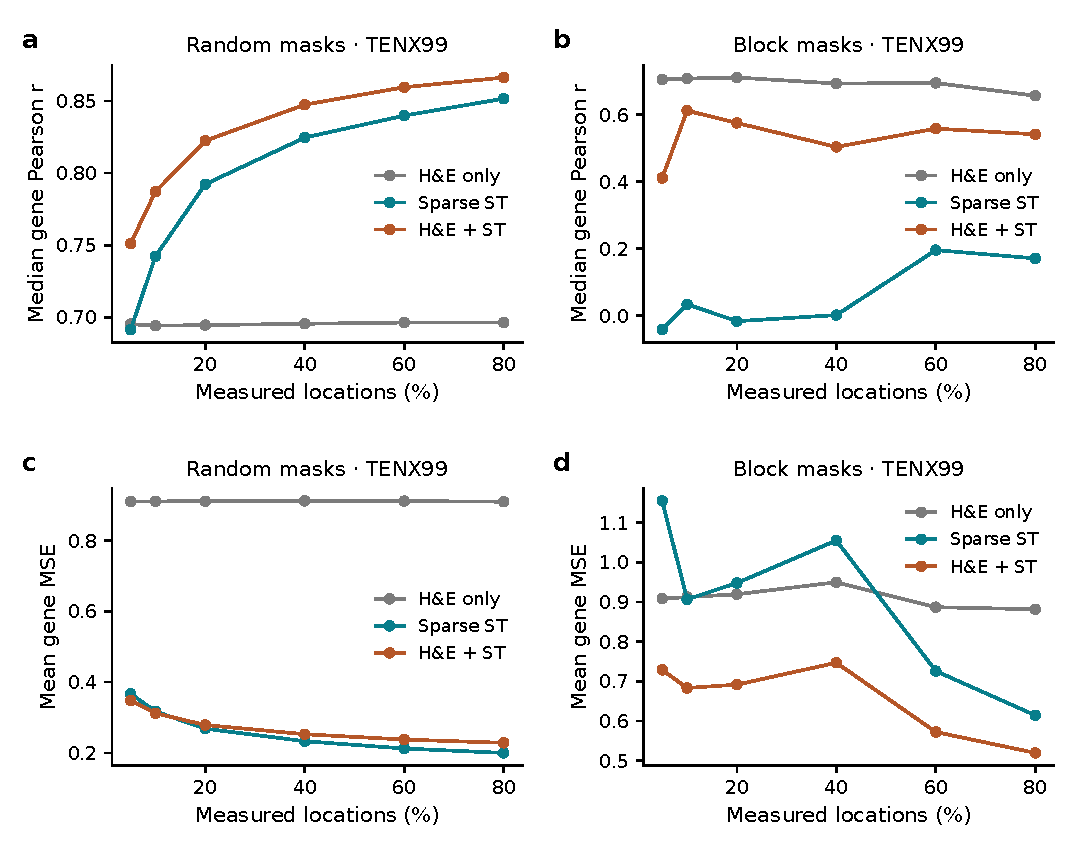
\includegraphics[width=\textwidth,height=0.60\textheight,keepaspectratio]{figures/Figure3.pdf}
\caption{\textbf{Development reconstruction depends on molecular coverage and masking regime.} Results are from the single primary development patient, TENX99, using the frozen 50-gene panel and ResNet18 representation. \textbf{a,c,} Distributed random observation. \textbf{b,d,} The earlier development block-mask regime. Panels a and b show median gene Pearson correlation; panels c and d show mean gene MSE across measurement fractions. The image-only, selected molecular interpolation and fixed fusion curves summarize three frozen mask replicates per condition; curves are means over masks, not patient confidence intervals. Targets and error units are unchanged across methods. The development block masks differ from the external V2 forbidden-region protocol and should not be treated as directly equivalent geometry tests. At 20\% distributed coverage, fusion has higher correlation than interpolation but slightly higher MSE, illustrating that spatial association and calibration are distinct properties. The image-only comparator receives no observed molecular anchors.}
\label{fig:development}
\end{figure}


In the fresh Wu evaluation, the median of patient-level median gene correlations at 20\% distributed coverage was 0.359 for spatial interpolation and 0.059 for image-only prediction (Fig.~\ref{fig:wu}). Corresponding MSEs were 0.0987 and 2.9155, and mean absolute errors (MAEs) were 0.2179 and 1.5578. All three evaluation patients favored interpolation over the frozen image predictor in correlation, MSE and MAE at every tested budget. The large error reduction is partly relative to an image predictor with substantial cross-platform scale and image-resolution mismatch; it should not be interpreted as accurate recovery of absolute transcript abundance or superiority over all image-based methods.

\begin{figure}[!htbp]
\centering
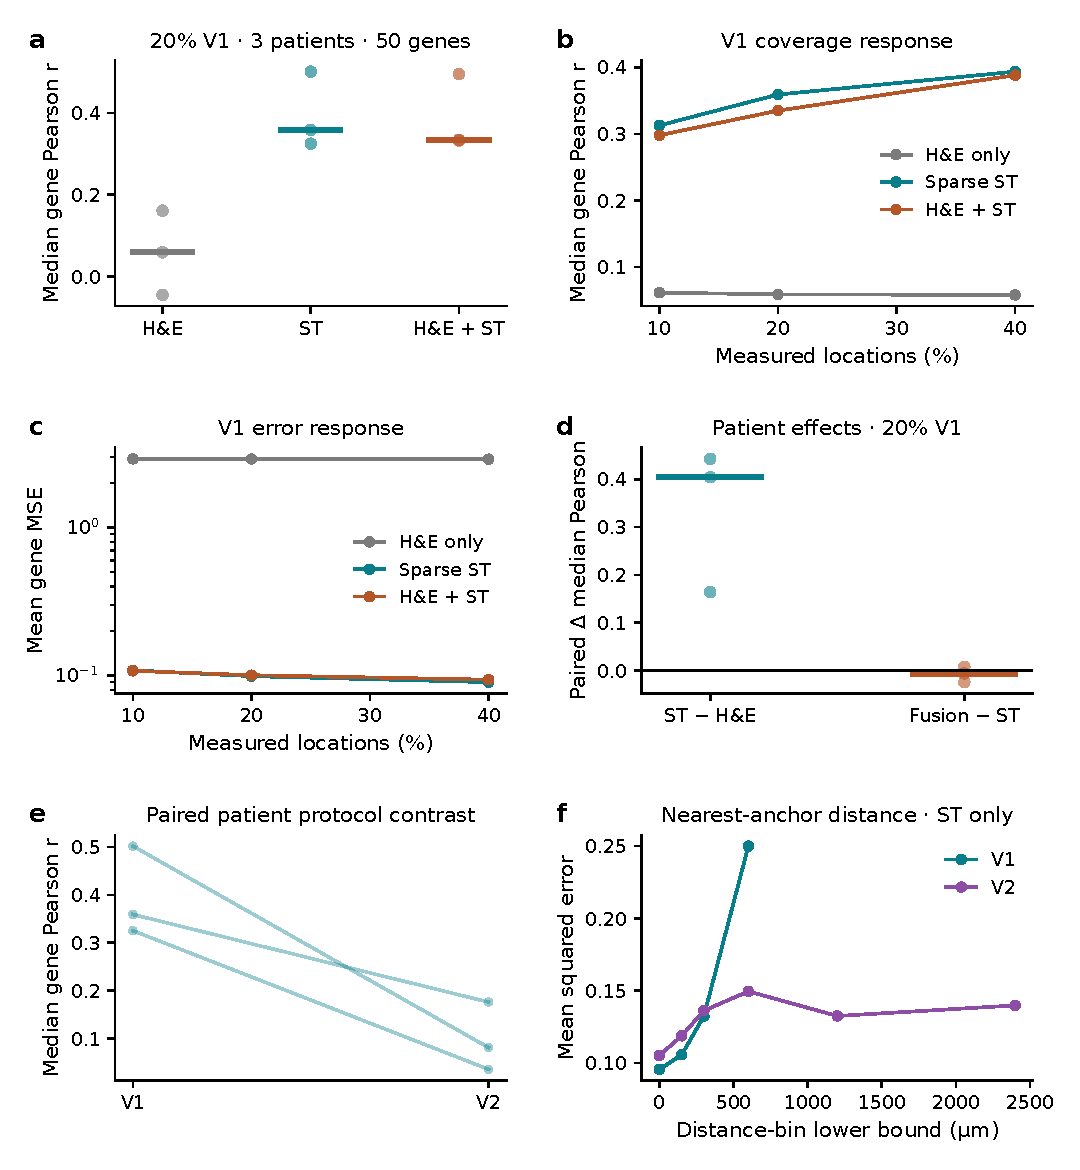
\includegraphics[width=\textwidth,height=0.70\textheight,keepaspectratio]{figures/Figure4.pdf}
\caption{\textbf{Fresh evaluation in three held-out Wu patients supports interpolation but not robust image fusion.} The frozen 50-gene panel was evaluated in patients 1160920F, CID4290 and CID44971, none of whom contributed to Wu calibration. \textbf{a,} Patient-level correlation summaries at 20\% distributed coverage. \textbf{b,c,} Median patient correlation and MSE across 10\%, 20\% and 40\% distributed coverage. \textbf{d,} Paired patient correlation effects for interpolation versus image-only prediction and fusion versus interpolation. \textbf{e,} Paired distributed (V1) and contiguous-region (V2) molecular correlations at 20\%. \textbf{f,} Distance-resolved molecular MSE at 20\%. Patient summaries average ten random mask seeds within geometry and then geometry means; cohort summaries are medians, not pooled spot estimates. Three fixed contiguous geometries are used for V2. Each patient is a biological replicate; seeds are not. V1 uses inverse-distance-squared interpolation and V2 uses a nearest-anchor mean, so panel e is a protocol contrast. The public image inputs contained only 15 or 25 native pixels per 112-\um{} patch, limiting conclusions about morphology. Error units are common development-standardized log1p counts.}
\label{fig:wu}
\end{figure}


The second fresh replication provided consistent support for the same comparison (Fig.~\ref{fig:bassiouni}). At 20\% distributed coverage, spatial interpolation achieved a median patient correlation of 0.416, MSE of 0.0923 and MAE of 0.2033. Image-only values were 0.075, 1.9673 and 1.2120. All 22 patients met the prespecified joint support criterion at each of the three budgets: a correlation gain of at least 0.02, relative MSE reduction of at least 2\%, and non-worsening MAE. This is a descriptive support criterion, not a significance test. Because interpolation receives measured expression from the evaluation section whereas the image-only model does not, the result establishes the utility of molecular anchors under the specified task rather than an equal-information algorithmic comparison.

\begin{figure}[!htbp]
\centering
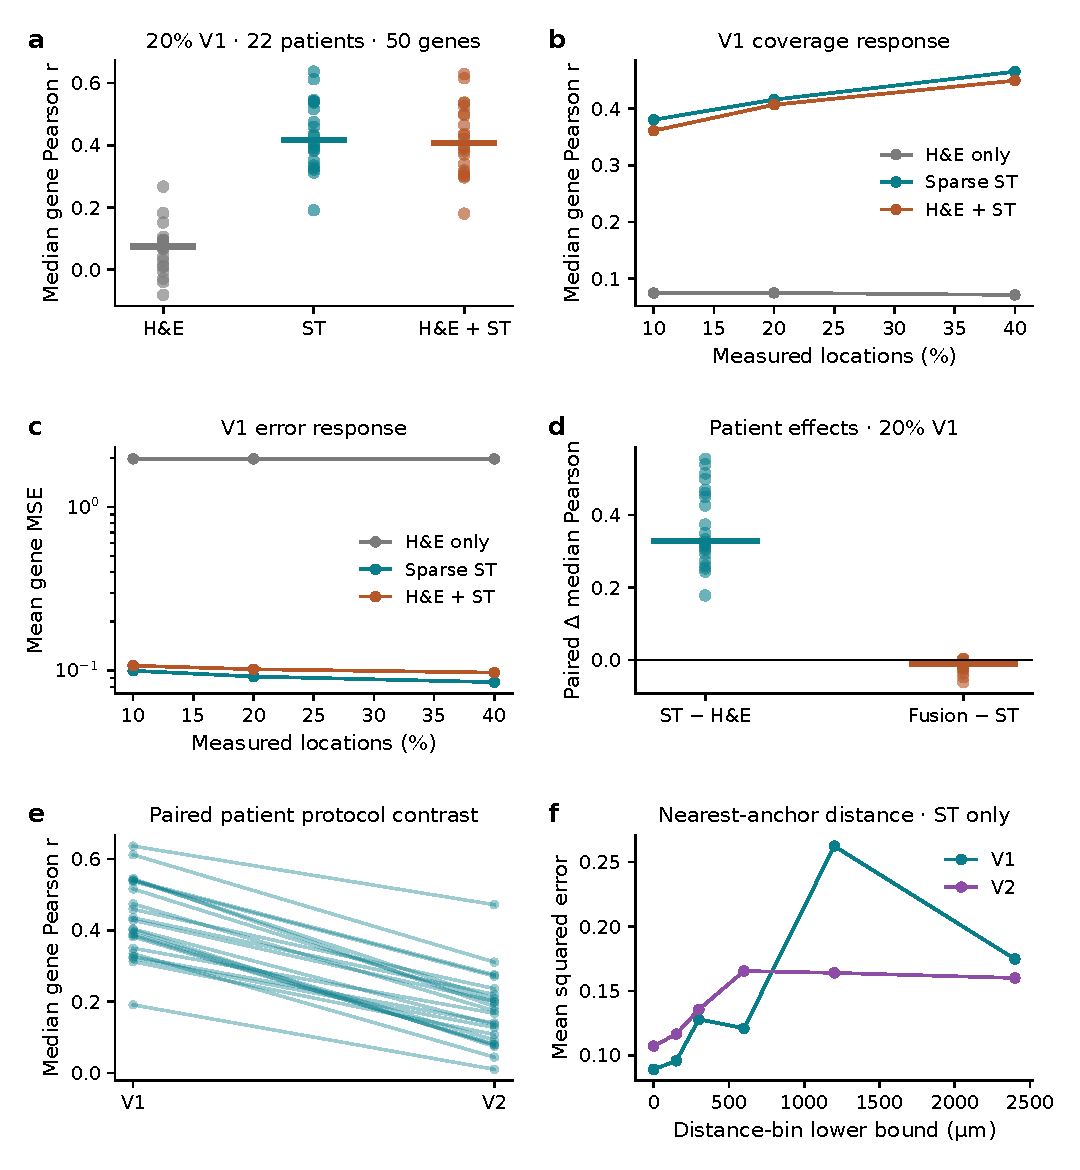
\includegraphics[width=\textwidth,height=0.70\textheight,keepaspectratio]{figures/Figure5.pdf}
\caption{\textbf{Independent 22-patient replication confirms the coverage response and weaker contiguous completion.} One first-numbered section per Bassiouni patient was selected before evaluation, yielding 30,003 locations and the same 50 primary genes. No patient from this study was used for new training or calibration. \textbf{a,} Patient correlation summaries at 20\% distributed coverage. \textbf{b,c,} Correlation and MSE across measurement fractions. \textbf{d,} Paired interpolation--image and fusion--interpolation correlation effects. \textbf{e,} Paired V1/V2 molecular correlations at 20\%. \textbf{f,} Distance-resolved molecular MSE at 20\%. Each patient summary averages ten mask seeds within geometry and then the three V2 geometry means where applicable; cohort curves use patient medians. All 22 patients improved in correlation and MSE between 10\% and 40\% V1 coverage and deteriorated in correlation, MSE and MAE under V2 relative to V1 at 20\%. V1/V2 differ in scoring support and interpolation weighting as well as missing-region design. Image fusion uses the frozen Wu calibration and 0.2 image weight. Public histology contained only 24--29 native pixels per 112-\um{} patch. Distance curves have varying occupied-bin support and are not calibrated uncertainty intervals. No p-values or patient confidence intervals are implied.}
\label{fig:bassiouni}
\end{figure}

\begin{table}[!htbp]
\caption{\textbf{Reconstruction at 20\% distributed measurement coverage.} Each entry is a cohort median of patient-level summaries after averaging mask seeds within geometry and geometries within patient, except that the development row represents the single primary patient. Pearson $r$ is the median correlation across panel genes; MSE and MAE are patient means across genes and hidden locations before the cohort median. All methods within a cohort use identical target units and observation masks. Different gene panels and assay count distributions preclude treating these values as a pooled cross-cohort ranking. Fusion rules and their calibration are frozen but differ between the development and external protocols; see Methods and Supplementary Information. The image-only branch has no same-section molecular anchors.}
\label{tab:performance}
\centering\small
\begin{tabularx}{\textwidth}{@{}Yrrlrrr@{}}
\toprule
Cohort & $n$ & Genes & Method & Pearson $r$ & MSE & MAE \\
\midrule
Development & 1 & 50 & Image only & 0.695 & 0.9110 & 0.7606 \\
 &  &  & Spatial interpolation & 0.792 & 0.2684 & 0.3904 \\
 &  &  & Fixed fusion & 0.822 & 0.2787 & 0.4173 \\
\addlinespace[5pt]
HER2ST, zero-shot & 8 & 40 & Image only & 0.143 & 4.3665 & 1.9376 \\
 &  &  & Spatial interpolation & 0.194 & 0.0680 & 0.1730 \\
 &  &  & Fixed fusion & 0.255 & 0.3481 & 0.5153 \\
\addlinespace[5pt]
Wu, fresh & 3 & 50 & Image only & 0.059 & 2.9155 & 1.5578 \\
 &  &  & Spatial interpolation & 0.359 & 0.0987 & 0.2179 \\
 &  &  & Fixed fusion & 0.335 & 0.1002 & 0.2321 \\
\addlinespace[5pt]
Bassiouni, fresh & 22 & 50 & Image only & 0.075 & 1.9673 & 1.2120 \\
 &  &  & Spatial interpolation & 0.416 & 0.0923 & 0.2033 \\
 &  &  & Fixed fusion & 0.407 & 0.1022 & 0.2288 \\
\bottomrule
\end{tabularx}
\end{table}


\subsection{Increasing distributed coverage improved reconstruction consistently}
Increasing the fraction of observed locations improved distributed reconstruction in both fresh cohorts (Supplementary Table~S9). Across the Bassiouni patients, median patient correlations at 10\%, 20\% and 40\% coverage were 0.380, 0.416 and 0.465; MSEs were 0.1001, 0.0923 and 0.0852. Every patient showed higher correlation and lower MSE at 40\% than at 10\%. The Wu cohort showed the same directional pattern in all three patients, with correlations of 0.313, 0.359 and 0.393 and MSEs of 0.1080, 0.0987 and 0.0899.

These curves describe the tested measurement fractions and do not identify a universally sufficient sampling budget. Coverage denotes the fraction of retained spatial locations whose complete expression vectors are revealed, not the fraction of tissue area assayed or a proportional reduction in experimental cost. Random sampling used nested anchor sets, but the hidden evaluation set also changes with coverage. The observed improvements therefore apply to the frozen budget-specific reconstruction protocols rather than to an identical set of targets at every budget. Label-free spatial coverage sampling was retained as a secondary analysis; earlier sampling comparisons had not established a reproducible advantage for difficult contiguous missing regions (Supplementary Fig.~S8).



\subsection{Contiguous regional completion exposed substantially weaker spatial prediction}
Under the contiguous missing-region protocol, reconstruction quality deteriorated across the fresh cohorts (Figs.~\ref{fig:wu} and \ref{fig:bassiouni}; Supplementary Table~S9). At 20\% coverage in the Bassiouni cohort, median patient correlation decreased from 0.416 for distributed interpolation to 0.171 for regional completion, while MSE increased from 0.0923 to 0.1496 and MAE from 0.2033 to 0.2624. All 22 patients deteriorated in all three measures. The median paired correlation change was $-0.267$, and the median paired relative MSE increase was 52.8\%. The latter is not the ratio calculated from separate cohort medians.

The Wu cohort showed a similar limitation: median patient correlation under the contiguous protocol was 0.0815, compared with 0.359 for distributed interpolation. Every patient had higher error and lower correlation. These results show that a favorable distributed-masking score does not imply equally reliable recovery across a large unmeasured region.

This contrast must nevertheless be interpreted at the protocol level. Distributed evaluation used inverse-distance-squared interpolation and scored all hidden locations; regional evaluation used a nearest-anchor mean and scored the designated contiguous region only. Thus the comparison changes the interpolation rule, the spatial arrangement of observed locations and the composition of the scored tissue. It does not isolate a causal effect of geometry. Moreover, a withheld region can lie inside the convex hull of observed anchors. We use ``contiguous extrapolation'' only as an operational description of extending predictions into a region without molecular observations, not as proof of geometric out-of-support extrapolation.

\subsection{Anchor distance was informative but did not define a universal reliability cutoff}
Distance-resolved error summaries complemented the panel-level results and spatial error maps (Fig.~\ref{fig:geometry}). In the Bassiouni cohort at 20\% coverage, the farthest occupied distance bin had higher MSE than the nearest bin in 15 of 22 patients for distributed interpolation and 20 of 22 for contiguous regional completion. Strictly increasing occupied-bin MSE curves occurred in only 6 and 13 patients, respectively. The Wu distributed curves increased across occupied bins in all three patients, whereas regional curves were nonmonotonic.

These heterogeneous patterns do not support a single extrapolation horizon applicable across patients, genes and missing-region designs. Distance bins contain different tissue locations and may differ in expression variance and tissue composition; remote bins can also contain relatively few observations. We therefore report bin support, omit empty bins and retain spatial error maps rather than assigning a universal distance cutoff (Supplementary Table~S7). The analysis describes an association between distance and reconstruction error without controlling all other sources of spatial heterogeneity.

\begin{figure}[!htbp]
\centering
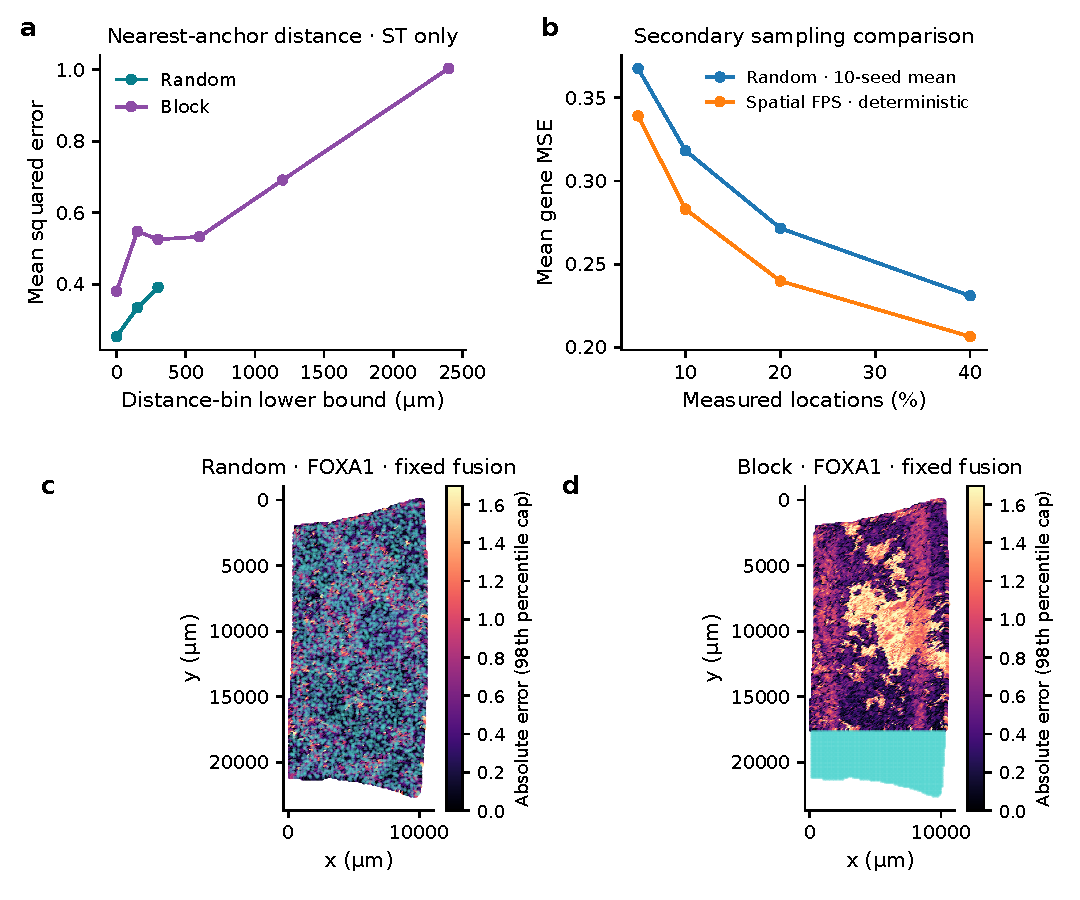
\includegraphics[width=\textwidth,height=0.60\textheight,keepaspectratio]{figures/Figure6.pdf}
\caption{\textbf{Spatial diagnostics reveal heterogeneous error beyond an overall prediction score.} Development results use TENX99 and the frozen 50-gene panel. \textbf{a,} Mean gene MSE versus nearest-anchor distance for molecular interpolation at 20\% coverage under distributed and development block masks; only occupied distance bins are shown. \textbf{b,} Development comparison of random and spatial farthest-point sampling, shown as MSE at matched measured-location budgets. These are descriptive single-patient sampling diagnostics, not a demonstration of universally optimal acquisition. \textbf{c,d,} Absolute-error maps for the preselected gene \textit{FOXA1}, fixed fusion, 20\% coverage and replicate 0 under random and block masks. Both maps use the same error scale, capped at the 98th percentile of the pooled preselected map-source values, which also include the archived capture-window condition; no locations are removed. Missing-region shape, available anchors and scored tissue differ between the maps. The figure illustrates why distance-bin support and spatial errors should accompany global correlation and why development geometry findings require independent evaluation.}
\label{fig:geometry}
\end{figure}

\FloatBarrier

\subsection{Frozen image fusion did not provide a reproducible external advantage}
The benefit of access to molecular anchors did not imply a benefit from adding the tested image prediction to those anchors. In the Bassiouni cohort at 20\% distributed coverage, fixed fusion yielded a median patient correlation of 0.407, MSE of 0.1022 and MAE of 0.2288, compared with 0.416, 0.0923 and 0.2033 for interpolation alone. Fusion increased correlation in only 3 of 22 patients and improved neither MSE nor MAE in any patient. Median paired correlation change was $-0.0108$, with a median paired relative MSE increase of 10.7\%. In the Wu cohort, only one of three patients improved in correlation and none improved in either error measure.

HER2ST transportability analyses had already exposed a substantial image/fusion calibration problem (Supplementary Figs.~S1 and S9). Recalibration during subsequent development reduced scale-related error, but selected fusion rules did not establish robust joint correlation and error improvements (Supplementary Fig.~S10). The final replication deliberately retained the Wu-derived calibration object and the fixed 0.2 image weight rather than adapting to Bassiouni outcomes. Together with external image downsampling, this restricts the conclusion to the frozen models and available inputs; it does not establish that high-resolution histology cannot improve a differently designed reconstruction method.

A separate invariance check clarified what target scaling could establish. Per-gene affine transformation followed by normalized linear interpolation and inverse transformation is algebraically equivalent to interpolation in the original target space. The molecular ``harmonized'' and unharmonized predictions consequently agreed to numerical precision. We did not count them as distinct algorithms or attribute improved molecular interpolation to this transformation (Supplementary Note: affine interpolation identity).

\subsection{Controls and provenance audits bounded the interpretation of the results}
Anchor-expression and anchor-position assignment permutations degraded molecular reconstruction in the predefined control cases, supporting dependence on the correct relationship between measured expression and location. These controls are related disruptions of the same association rather than independent mechanistic tests. Image permutation did not provide comparable evidence for a useful image contribution (Supplementary Figs.~S11 and S12; Supplementary Table~S4). Earlier morphology, graph-topology and encoder experiments were retained transparently and did not justify claims that exact graph topology was essential (Supplementary Figs.~S3--S7).

The second replication produced 2,904 clean and 18 control bundles, containing 8,766 method predictions. All 17,532 hidden-label NaN/random corruption comparisons were invariant. The recorded audit reproduced 8,766 predictions and 35,064 per-gene metric arrays exactly and reconstructed 968 label-free mask trajectories. These checks establish computational traceability within the frozen workflow; they do not replace independent biological replication or remove limitations of the target representation (Supplementary Tables~S5 and S6).

\section{Discussion}
\paragraph{Potential measurement-cost implication.}
The 20\% coverage protocol reveals molecular expression at one fifth of retained spatial locations, equivalent to fivefold fewer measured locations than complete profiling in the retrospective masking design. If the location-dependent expenditure is proportional to the number of assayed locations, its variable component could be reduced fivefold. With fixed cost $C_0$, variable cost $c$ per location and $N$ full-coverage locations, however, the ratio is
\begin{equation}
\frac{C_{\mathrm{full}}}{C_{20\%}}=\frac{C_0+cN}{C_0+0.2cN}\leq 5.
\label{eq:cost_ratio}
\end{equation}
The study did not implement selective capture or measure laboratory expenditure, and the inequality does not claim fivefold reduction in total assay costs. Coverage describes the retained location count, not an experimentally validated reduction in tissue area, sequencing burden or platform price. Prospective acquisition and outcome-specific accuracy requirements would be necessary to establish realized savings.


This study shows that a simple, frozen spatial interpolation protocol can recover part of the variation in a predefined expression panel when molecular measurements are available at distributed locations in the same tissue section. The direction of benefit over the frozen image-only comparator was consistent in two fresh breast cancer studies, including all 22 patients in the larger replication. Increasing measured-location coverage improved correlation and reduced error, whereas contiguous regional completion remained substantially weaker. The contribution is the explicit separation of tissue-context representation learning from observation-constrained molecular transport, together with multi-cohort characterization of reconstruction reliability; we do not claim transcriptome-wide recovery or a newly learned long-range GNN.

The comparison with histology requires particular care. Molecular interpolation uses patient-specific observations from the evaluation section and therefore has access to information unavailable to the image-only model. Its advantage demonstrates the practical value of these anchors but does not establish superiority over all histology-based prediction methods. Prior image-based and multimodal approaches address different training and inference settings\cite{he2020,monjo2022,bergenstrahle2022,liu2026}. The appropriate test of incremental morphology in our setting was fusion versus interpolation. That test did not show a reproducible benefit. Low-resolution public images, a generic ImageNet representation and transported calibration constrain the comparison; a comprehensive benchmark of native-resolution pathology models was outside the frozen replication protocol.

The contiguous missing-region results make the evaluation design as important as the average score. A method that interpolates between nearby measurements can perform poorly when observations are absent from a substantial tissue region. This is consistent with the broader need to match validation structure to the intended prediction task in spatially dependent data\cite{roberts2017}. However, our V1/V2 protocols also differ in interpolation family and scored locations. A future factorial study holding the interpolation rule and evaluation support fixed would be needed to estimate the isolated contribution of missing-region geometry. In the present analysis, the defensible conclusion is that the entire contiguous-completion protocol is harder, not that geometry alone explains the measured decline.

Distance-to-anchor summaries expose additional heterogeneity but are not calibrated uncertainty estimates. The absence of a universal monotonic curve suggests that distance alone is insufficient to determine where a reconstructed expression value is trustworthy. Reconstruction may also be affected by variation in the target field and the composition of the scored locations. Uncertainty-aware approaches such as TISSUE illustrate why uncertainty in predicted expression matters for downstream analyses\cite{sun2024}; we did not implement that framework or claim calibrated intervals here. Regional errors, low-support bins and patient-specific failures should remain visible before reconstructed values are used for differential expression, cell-state interpretation or other biological analyses.

Cross-platform scale differences present a distinct challenge. A common numerical transformation does not make targeted in situ counts and sequencing-based capture-spot counts biologically interchangeable. Capture support, depth and composition remain different even after values are centered and scaled. The observed reduction in image/fusion error during HER2ST calibration development should therefore not be confused with a validated improvement in molecular interpolation. The affine identity shows why the latter comparison is unidentifiable for the specified normalized weighted average. It also provides a useful implementation check: negligible numerical rank differences should not be interpreted as biological gains.

Several limitations define the scope of the study. The primary panel was selected in development and contained 50 genes, with only 40 shared in HER2ST. The results do not establish recovery of unmeasured genes or an entire transcriptome. Missingness was simulated by withholding existing measurements, not created through a prospective reduced-assay experiment. Reported coverage is a proportion of retained locations and does not translate directly to tissue area, sequencing expenditure or financial savings. Patient numbers were small in the first fresh validation, and all cohorts were breast tissue. External images were downsampled and the frozen fusion rule was not optimized for them. We also did not benchmark a comprehensive set of spatial statistical or modern histology-to-expression methods under equal information access. Consequently, the current evidence should not be read as state-of-the-art superiority or clinical utility.

The sequential design offers a complementary strength. Development, inspected transportability cohorts and fresh evaluation cohorts were kept distinct, and mixed results were retained rather than used to retroactively revise the external protocol. Technical replay, mask provenance and hidden-label corruption checks reduce the risk that an apparent reconstruction benefit arises from leakage. These safeguards are especially important when measurement masks expose expression from the evaluation tissue itself. Nevertheless, the decision rules and repeated development analyses remain part of an iterative research process rather than a substitute for prospective experimental confirmation.

Overall, sparse molecular anchors provided useful reconstruction under distributed sampling, with a consistent coverage response across fresh cohorts. The same evidence delineated weaker contiguous regional completion and a lack of reproducible benefit from the tested image fusion. Reporting measurement coverage, missing-region design, anchor distance, calibration behavior and patient-level effects together gives a more informative account of reliability than a single pooled prediction score.

\section{Methods}
\subsection{Data sources and analytical roles}
All experiments used previously released paired spatial expression and histology data. The four development samples were obtained through HEST\cite{jaume2024}: NCBI783 and NCBI785 were the training patients, TENX95 was the validation patient and TENX99 was the primary development evaluation patient. The cohort comprised 7,015 training locations, 7,760 validation locations and 20,761 primary evaluation locations. Earlier conditional leave-one-patient-out analyses reused frozen gene panels and development-selected configurations and were interpreted as sensitivity analyses, not unbiased external cross-validation.

HER2ST\cite{andersson2021} contributed one patient-specific section for each of A1--H1. Initial evaluation was followed by patient-disjoint calibration development using the same inspected cohort; these two analytical roles are distinguished throughout. In the Wu local Visium cohort\cite{wu2021}, patients 1142243F, CID4465 and CID4535 supplied calibration statistics, and patients 1160920F, CID4290 and CID44971 remained held out. The fresh Bassiouni cohort was obtained from GSE210616\cite{bassiouni2023}. The source study includes 43 sections from 22 patients. We selected the first numbered section for every published patient from metadata before target evaluation, yielding BASS\_P01--P09, P11--P15 and P17--P24. Gaps in identifiers reflect source numbering rather than outcome-dependent exclusion. The source study's own reference and validation groups were not used as calibration groups in this reconstruction study.

Metadata, repository identifiers, prior-use records and available asset hashes were checked to exclude reused or reprocessed development samples. Such checks support cohort independence but cannot conclusively establish patient identity across unrelated anonymized repositories. Cohort roles and sample counts are summarized in Table~\ref{tab:cohorts}; identifiers and exact panels are supplied in Supplementary Tables~S1 and S2.

\subsection{Expression targets and preprocessing}
The primary panel contained the 50 genes ranked using development-training expression variance; ranking did not use evaluation expression. The development assay provided 280 harmonized biological genes, and larger 250- and 280-gene settings were used in earlier development analyses. The primary fresh studies retained all 50 genes. HER2ST retained the frozen 40-gene intersection without replacing missing genes. The optional 278/280 intersection in the Bassiouni metadata was not used to claim a secondary whole-transcriptome experiment.

For the second replication, the source filtered feature-barcode H5 files, tissue positions, scale-factor JSON files and tissue images were acquired for each selected section. Barcode joins and published in-tissue flags defined included locations. No new expression-derived quality threshold, tissue-class annotation or deconvolution output was used to select evaluation locations. Counts were checked for finite, nonnegative integer values. For count $c_{ig}$ at location $i$ and gene $g$, the evaluation target was
\begin{equation}
 y_{ig}=\frac{\log(1+c_{ig})-\mu_g^{\mathrm{dev}}}{\sigma_g^{\mathrm{dev}}},
 \label{eq:target}
\end{equation}
where the centering and scaling constants were the pooled location mean and population standard deviation frozen from development-training patients; a standard deviation below $10^{-8}$ was replaced by 1. No destination library-size or capture-area correction was fitted. Identical target units were used for all methods within each comparison. These common mathematical units do not imply cross-platform calibration of absolute molecular abundance. Supplementary Fig.~S2 summarizes cross-cohort patterns without pooling panels; the gene-level results are provided in Supplementary Table~S3.

\subsection{Spatial registration and image acquisition}
Visium array coordinates were mapped to image coordinates by a least-squares fit to the source hexagonal lattice with 100-\um{} spacing. Coordinate residuals, image scale and anisotropy were checked against the frozen qualification settings, and overlays were inspected before outcome evaluation. These tests concern location consistency and do not establish cell-level registration. Images were not super-resolved.

The Wu and Bassiouni images contained only 15/25 and 24--29 native pixels, respectively, across the nominal 112-\um{} patch width. Resizing does not recover morphology absent from these public inputs. Image quality was therefore recorded as a limitation of the image comparator, not as a restriction on spatial interpolation that uses only coordinates and observed expression.

\subsection{Neural image predictor and reconstruction architecture}
The reconstruction framework combined a frozen neural image predictor with a separate coordinate-based molecular interpolation branch (Fig.~\ref{fig:overview}). Both predicted the same ordered 50-gene panel. Molecular interpolation used spatial coordinates and observed expression; the final fusion was a fixed weighted average, with no additional neural layers fitted in the fresh replication experiments.

At each external location, an RGB patch covered a nominal $112$-\um{} square, rounded to the available native pixels. The patch was resized with LANCZOS to $224\times224$ pixels. The torchvision \texttt{IMAGENET1K\_V1} preprocessing then resized the shorter side to 256 pixels using bilinear interpolation, took a central $224\times224$ crop, rescaled intensities to $[0,1]$, and normalized RGB channels using means $(0.485,0.456,0.406)$ and standard deviations $(0.229,0.224,0.225)$. The second resize and central crop were retained explicitly; $112$~\um{} denotes the nominal extracted patch, rather than the final uncropped field seen by the network. Development embeddings used the supplied $224\times224$ HEST patches with the same torchvision transform. No stain normalization, random image augmentation or encoder fine-tuning was applied.

The frozen ResNet18\cite{he2016} comprised a $7\times7$ convolutional stem with stride 2, batch normalization, a rectified-linear activation and $3\times3$ max pooling with stride 2, followed by four residual stages. The stages contained two basic blocks each, with channel widths 64, 128, 256 and 512. Each block used two $3\times3$ convolutions with batch normalization and a rectified-linear activation after the first convolution and after shortcut addition. Identity or projected shortcuts matched the feature dimensions. Global average pooling produced a 512-dimensional vector; the original ImageNet classifier was replaced by the identity operation. All encoder parameters and batch-normalization statistics remained fixed during feature extraction.

Each expression head was a one-hidden-layer MLP with the exact sequence
\begin{equation}
512 \xrightarrow{\mathrm{linear}}256
\xrightarrow{\mathrm{GELU}}256
\xrightarrow{\mathrm{dropout}\;(0.1)}256
\xrightarrow{\mathrm{linear}}50,
\label{eq:head}
\end{equation}
where GELU denotes the Gaussian error linear unit. Both linear layers included biases and used the default PyTorch initialization, uniform on $[-1/\sqrt{d_{\mathrm{in}}},1/\sqrt{d_{\mathrm{in}}}]$. The output was linear, with no nonnegativity constraint. Each head contained 144,178 trainable parameters. Feature-wise centering and scaling, $S_x$, were fitted to the pooled 7,015 training locations from NCBI783 and NCBI785. A separate per-gene scaler, $S_y$, was fitted to their already normalized expression targets. Both used population standard deviations, replacing scales below $10^{-8}$ with 1. If $f_{\theta_s}$ denotes the head trained with seed $s\in\{0,1,2\}$ and $\phi_{\mathrm{R18}}$ the frozen encoder, the image prediction in the common target units was
\begin{equation}
\widehat{\boldsymbol y}^{\mathrm{image}}_i
=\frac{1}{3}\sum_{s=0}^{2}
S_y^{-1}\!\left[f_{\theta_s}\!\left(S_x\!\left(\phi_{\mathrm{R18}}(x_i)\right)\right)\right].
\label{eq:image_ensemble}
\end{equation}
Dropout was disabled at inference. The three inverse-scaled predictions were averaged without fitting ensemble weights.

Heads minimized mean squared error in the additionally standardized target space using AdamW, learning rate $10^{-3}$, weight decay $10^{-4}$, $(\beta_1,\beta_2)=(0.9,0.999)$ and $\epsilon=10^{-8}$. Weight decay applied to all head parameters, including biases. Each epoch shuffled the training locations into minibatches of 512, retaining the final partial batch, for at most 80 epochs. Training used CPU float32 computation and no learning-rate scheduler. Early stopping used the TENX95 validation patient: an improvement required validation MSE to decrease by more than $10^{-4}$, and training stopped after 10 consecutive epochs without such an improvement. The best qualifying parameters were restored. Hidden widths $\{128,256\}$ and dropout probabilities $\{0,0.1\}$ were compared at seed 0; the configuration with the highest validation median gene Pearson correlation was selected, with lower validation MSE breaking ties. This configuration-selection criterion was distinct from the within-fit stopping criterion. The selected width-256, dropout-0.1 heads were fitted with seeds 0, 1 and 2; their retained epochs were 12, 11 and 12, respectively. No external patient was used to select or refit these heads.

The molecular branch used up to 16 observed anchors and the weights in Eq.~\ref{eq:interp}. Fusion combined its output with the calibrated image prediction using fixed molecular and image weights of 0.8 and 0.2 (Eq.~\ref{eq:fusion}). The calibration established from development-training and Wu calibration patients was transported unchanged to Bassiouni.

\subsection{Graph construction from physical tissue geometry}
For every tissue section, retained locations are vertices $V=\{1,\ldots,N\}$ with physical positions $p_i\in\mathbb{R}^2$ and frozen image embeddings $x_i\in\mathbb{R}^{d}$. Candidate graphs $G=(V,E)$ were computed without expression measurements. The symmetrized six-nearest-neighbor construction connects $i$ and $j$ if either is among the other's six nearest locations and their separation is within 250~\um{}. Radius graphs use a 150- or 250-\um{} distance threshold. Delaunay triangulation provides an alternative geometry-induced candidate edge set, capped at 250~\um{}. Edges are undirected and binary, and isolated vertices are retained. Different edge definitions produce different contextual neighborhoods at the same spatial coordinates (Fig.~\ref{fig:graph_architecture}).

The graph-context models operate on $X=[x_1,\ldots,x_N]^\top$ after fitting-data standardization. With adjacency $A$, self-augmented adjacency $\widetilde A=A+I$ and its diagonal degree matrix $\widetilde D$, our fixed mean and GCN aggregators are $P=\widetilde D^{-1}\widetilde A$ and $Q=\widetilde D^{-1/2}\widetilde A\widetilde D^{-1/2}$. Mean-GraphSAGE concatenates the original embedding with its separate-neighbor mean $R X$, where $R=D^{-1}A$ and zero-degree rows of $R$ are zero. The three resulting features $PX$, $QX$ or $[X,RX]$ are passed through a trainable regression head, rather than through stacked learned message-passing layers. This is a single-step contextual representation, consistent with established graph aggregation principles\cite{gilmer2017,kipf2017,hamilton2017}.


\subsection{Experimental setup: shared heads and training}
\label{sec:experiments}
The supporting image and graph comparisons used the development split described in the main Methods: NCBI783 and NCBI785 for fitting, TENX95 for validation and TENX99 for the primary evaluation. The image encoders remained frozen. Each trainable multilayer perceptron (MLP) had one hidden fully connected layer, a Gaussian error linear unit (GELU), dropout and a linear gene-output layer:
\[
 f(U)=\operatorname{Dropout}_{p}\!\left[\operatorname{GELU}(UW_1+b_1)\right]W_2+b_2.
\]
The input $U$ was a local image embedding or a fixed aggregate of embeddings, as specified below. Feature and target means and population standard deviations were estimated from fitting patients only; scales below $10^{-8}$ were replaced by one. The additional target standardization used to train the head was inverted before scoring in the common development target units. For graph predictors, the local embeddings were standardized before aggregation.

All MLPs minimized mean squared error with AdamW, learning rate $10^{-3}$, weight decay $10^{-4}$ and minibatch size 512. Training used a new random ordering of fitting rows each epoch, at most 80 epochs and validation-MSE early stopping with patience 10 and minimum improvement $10^{-4}$. The parameters at the best qualifying validation epoch were retained, and dropout was disabled for prediction. The three training seeds were 0, 1 and 2; hyperparameter candidates were evaluated using seed 0. No learning-rate schedule or auxiliary loss was used. Computation used CPU float32 tensors and four threads with deterministic PyTorch algorithms enabled.

The initial local comparison in Supplementary Fig.~S3 selected hidden width from $\{128,256\}$ and dropout from $\{0,0.1\}$ by the lowest validation MSE. For 50 genes, the selected architecture was $512\rightarrow128\rightarrow50$ with dropout 0.1. The ridge baseline used an intercept and a Cholesky solver, with penalty selected from $\{10^{-4},10^{-3},10^{-2},10^{-1},1,10,100\}$ by the highest validation median gene Pearson correlation, breaking ties by lower MSE and then smaller penalty; the selected 50-gene penalty was 100. Training-target and training-embedding permutations disrupted pairing within the fitting data; validation and evaluation data were unchanged.

The representation comparison in Supplementary Fig.~S6 used the same four width/dropout candidates but selected the highest validation median gene Pearson correlation, with lower MSE as the first tie-breaker. Both ResNet18 and Phikon selected width 256 and dropout 0.1 for 50 genes. Thus the initial local predictor in Supplementary Fig.~S3 and the ResNet18 predictor used in the representation comparison and final sparse pipeline have different selected widths. The latter predictor is described in the main Methods. The representation comparison also evaluated ridge penalties $\{0.1,1,10,100,1000\}$; both encoders selected 1000 for 50 genes. Equal width and search budget did not imply equal parameter count because the input dimensions differed.

Conditional leave-one-patient-out sensitivity fits used the remaining three development patients, refitted feature and head-target scalers on those patients, retained the primary-selected hyperparameters and used fixed epoch counts without early stopping on the held-out patient. For the 50-gene heads, these counts were 14 for the initial MLP, 14 for mean pooling and GCN, 7 for GraphSAGE, 12 for the representation-comparison ResNet18 head and 1 for the Phikon head. These were rounded medians of the corresponding primary fits' best epochs. Since the configurations and underlying target definition had already been selected during development, these fits are conditional sensitivity analyses.

\subsection{Coordinate-based graph construction and GNN representation learning}
\label{sec:graph_methods}
Graphs were constructed independently within each section from physical coordinates, without expression labels. The candidates were symmetrized six-nearest-neighbor adjacency capped at 250~\um{}, radius graphs at 150 or 250~\um{}, and Delaunay adjacency capped at 250~\um{}. Symmetrization takes the union of directed nearest-neighbor edges, so final degree need not equal six. The binary adjacency $A$ had no self edges. With $\widetilde A=A+I$, degree matrix $\widetilde D$ of $\widetilde A$, and degree matrix $D$ of $A$, the three fixed operators were
\[
 P=\widetilde D^{-1}\widetilde A,\qquad
 Q=\widetilde D^{-1/2}\widetilde A\widetilde D^{-1/2},\qquad
 R=D^{-1}A.
\]
For $R$, an isolated node has a zero neighbor aggregate. The input to the MLP was $PX$ for mean pooling, $QX$ for GCN and $[X,RX]$ for mean-GraphSAGE, where $X$ contains standardized frozen image embeddings and brackets denote concatenation. Each predictor therefore applies one fixed graph aggregation followed by the one-hidden-layer MLP defined above. No graph attention or learned adjacency was used.

Graph choice was selected at seed 0 by the highest validation median gene Pearson correlation, then lower MSE and deterministic graph-name order. All three 50-gene predictors selected capped Delaunay adjacency. Mean pooling and GCN used width 128; GraphSAGE used width 67 to approximately match the initial local head's parameter count after doubling the input dimension. With ResNet18, these models contain 72,114 and 72,075 trainable head parameters, respectively; all use dropout 0.1. Supplementary Table~S8 summarizes the selected dimensions.

The matched controls in Supplementary Fig.~S5 retained the GraphSAGE head and training settings. The self-only control used $[X,X]$. Vertex permutation preserved the graph's degree distribution, while double-edge rewiring preserved each node's degree. The additional distance-constrained rewiring preserved the numbers of physical edge lengths in $[0,175)$, $[175,250)$ and $[250,\infty)$~\um{}. Rewiring targeted five accepted swaps per edge, with limits of 100 attempts per edge for degree-only rewiring and 1,000 for distance-constrained rewiring; the latter used candidate endpoints within 275~\um{}. Five graph randomization seeds were crossed with the three model seeds. The Phikon spatial sensitivity comparison reused the selected graph, hidden widths and dropout: mean pooling used $768\rightarrow128\rightarrow50$, and GraphSAGE used $1536\rightarrow67\rightarrow50$, with true and degree-plus-length-matched graphs. These inherited widths do not constitute exact parameter matching between encoders.

\subsection{Pathology foundation representation comparison}
Phikon used the public \texttt{owkin/phikon} ViT-B/16 model, pinned to \href{https://huggingface.co/owkin/phikon/tree/057cc0295895c2df3dd7681a89680da6015cbefe}{revision \texttt{057cc0295895}}. Its 12-layer transformer produced the 768-dimensional final-layer-normalized classification-token representation, without a pooler. The official \texttt{ViTImageProcessor} processed the same RGB patches as the ResNet18 analysis: $224\times224$ pixels, rescaling by $1/255$ and ImageNet channel means and standard deviations. There was no recropping, stain normalization or augmentation. Extraction used the model in evaluation mode with frozen weights, float32 precision, batches of 16 and eight CPU threads (Transformers 4.57.3, PyTorch scaled dot-product attention). The head and validation selection were as specified above; the encoder was not fine-tuned.

\subsection{Sparse molecular graph reconstruction and residual correction}
The learned-propagation model in Supplementary Fig.~S7 is a gene-specific ridge residual correction using fixed graph summaries. Its image prediction $H$ is the equal average of the three frozen local MLP predictions from the representation comparison. Let $o$ be the observed-location indicator and $Z$ the expression matrix containing permitted observed vectors and zeros elsewhere. A self-inclusive row-normalized operator $P$ was constructed from the symmetrized six-nearest-neighbor graph capped at 250~\um{}. The observed masses and molecular messages were
\[
 m^{(1)}=Po,\quad m^{(2)}=P^2o,\qquad
 V^{(1)}_{ig}=\frac{(PZ)_{ig}}{\max(m^{(1)}_i,10^{-6})},\quad
 V^{(2)}_{ig}=\frac{(P^2Z)_{ig}}{\max(m^{(2)}_i,10^{-6})}.
\]
Image features were standardized on fitting patients and reduced to eight whitened principal components with randomized singular-value decomposition and random seed 0. Denote these components by $X_{\rm PCA}$. The 29 shared covariates at each location were $X_{\rm PCA}$, $PX_{\rm PCA}$, $P^2X_{\rm PCA}$, $o$, $m^{(1)}$, $m^{(2)}$, $\log(1+d_1/100)$, and the fraction of the nearest 16 observed anchors lying within 300~\um{}, where $d_1$ is nearest-anchor distance in \um{}. Five further covariates for gene $g$ were the image prediction $H_g$, the fixed fusion prediction $F_g$, $Z_g$, $V^{(1)}_g$ and $V^{(2)}_g$. The resulting design has 34 covariates and an intercept for each gene.

Predictions were $\widehat y_g=F_g+\Phi_g\theta_g$, where the last column of $\Phi_g$ is one. Coefficients were fitted by
\[
 \underset{\theta_g}{\operatorname{argmin}}\;
 \left\|(y_g-F_g)-\Phi_g\theta_g\right\|_2^2
 +\alpha\left\|\theta_{g,1:34}\right\|_2^2.
\]
The intercept was unpenalized. Fitting sampled up to 256 hidden locations without replacement per training mask using that mask's seed; their expression entered only the supervised response. Masks covered 5, 10, 20, 40, 60 and 80\% of locations under random, block and capture-window sampling, with three replicates per condition. The penalty grid was $\{1,100,10000\}$, selected by mean validation MSE across masks with equal mask weights; both encoders selected $\alpha=10000$ for 50 genes. No additional expression scaler or auxiliary loss was introduced.

The underlying development fusion was $F=\lambda H+(1-\lambda)M$. Nearest-anchor mean interpolation selected $k$ from $\{1,4,8,16\}$; inverse-distance interpolation used up to 16 anchors and selected power from $\{1,2,3\}$. The stronger family and $\lambda\in\{0,0.25,0.5,0.75,1\}$ were chosen by mean validation MSE separately by panel and sampling geometry. For 50 genes, random sampling selected inverse-distance-squared interpolation and $\lambda=0.25$; block sampling selected the 16-anchor mean and $\lambda=0.5$; capture-window sampling selected inverse-distance-cubed interpolation and $\lambda=0.5$. These development settings differ from the final external fusion settings. Supplementary Fig.~S7 evaluates three permutation seeds on one random 20\% observation mask, with the fitted models unchanged. The plotted B1, B3 and B4 labels denote the frozen image predictor, fixed fusion and ridge residual correction, respectively.

\subsection{Patient-disjoint HER2ST calibration and fusion selection}
Supplementary Figs.~S1 and S10 use the same eight HER2ST patients and 40 shared genes. Four outer folds held out the pairs A1/B1, C1/D1, E1/F1 and G1/H1, respectively. Within each remaining six-patient set, target-mapping candidates were evaluated by leave-one-patient-out records: the mapping for an inner patient's predictions was estimated from the other five patients. The fixed source moments came from NCBI783 and NCBI785. The candidates were the unchanged target, per-gene mean/standard-deviation mapping and per-gene median/interquartile-range mapping. Each patient had equal total weight in moment or quantile estimates. An interquartile range below $10^{-8}$ fell back to the corresponding standard deviation, and a standard deviation below $10^{-8}$ was replaced by one. Source and destination moments were estimated separately. Image predictions were expressed in source-standardized coordinates, anchors in destination-standardized coordinates, and final errors were computed after mapping predictions back to common target units.

The target-mapping comparison retained fixed image weights 0.25 for V1 and 0.5 for V2. Selection used inner random-mask seeds 0--2 and four equally weighted conditions: V1 coverage 10, 20 and 40\%, and V2 coverage 20\%. Seeds and geometries were first averaged within patient and condition, then conditions within patient, then the six patients. Candidates within 0.005 of the highest mean patient median gene Pearson correlation were eligible; among these, the candidate with lowest common-unit MSE was selected. The mean/standard-deviation transform was selected in every fold; the corresponding outer mapping used moments estimated from all six outer-training patients.

The selected-fusion analysis then used the corresponding inner records to fit and select among four families: molecular interpolation alone; one global image weight from $\{0,0.1,\ldots,1\}$; 35 nondecreasing three-bin weight rules with weights from $\{0,0.1,0.25,0.5,1\}$ and nearest-anchor boundaries 300 and 600~\um{}; and a five-parameter sigmoid gate. All weights were shared across genes, regimes and budgets within an outer fold. The sigmoid gate was
\[
 w_i=\operatorname{sigmoid}(\beta_0+\widetilde q_i^\top\beta),\qquad
 \widehat y_i=M_i+w_i(H_i-M_i),
\]
where the four features before fitting-data standardization were $\log(1+d_1/200)$, $\log(1+\overline d_{16}/200)$, $\log(1+n_{600})$ and $\log(1+v)$: nearest-anchor distance, mean distance to up to 16 nearest anchors, the number of observed anchors within 600~\um{}, and mean across-gene variance among the neighboring observed vectors. The gate minimized common-unit squared error with equal patient/condition/run/location contributions, divided by each run's interpolation MSE floored at $10^{-8}$, plus $0.01\|\beta\|_2^2+10^{-6}\beta_0^2$. The same weights defined feature means and standard deviations. L-BFGS-B used initial coefficients $(-2,0,0,0,0)$, bounds $[-12,12]$, maximum 300 iterations, function tolerance $10^{-12}$ and gradient tolerance $10^{-7}$. No outer-patient outcomes entered fitting or candidate selection.

The same correlation-then-MSE rule selected the fusion family. The first three patient-pair folds selected global image weight 0.2; the G1/H1 fold selected the sigmoid gate. Outer evaluation used mask seeds 0--9. Supplementary Fig.~S10 reports these fold-selected rules, whereas Supplementary Fig.~S1 shows the fixed-fusion target-mapping comparison. Both remain calibration-development analyses of previously examined HER2ST patients.


The full-precision primary image feature scaler, target normalization and source-to-Wu calibration constants are supplied in \path{methods_data/}. The primary head settings and recorded software versions are provided there in machine-readable form. These constants specify the published transformations without refitting them.

\subsection{Development comparisons of local and contextual representations}
Development analyses compared an initial local MLP, neighborhood-mean pooling, and predictors using graph-convolutional\cite{kipf2017} or mean-GraphSAGE\cite{hamilton2017} representations (Supplementary Figs.~S3 and S4). The implemented graph predictors applied one fixed aggregation to frozen image embeddings, followed by a one-hidden-layer GELU MLP; they did not stack multiple trainable message-passing layers. Self-only, vertex-permuted, degree-rewired and degree-plus-edge-length-rewired controls tested whether gains depended on the true spatial adjacency (Supplementary Fig.~S5). The representation comparison used the 768-dimensional final classification-token representation from frozen Phikon ViT-B/16\cite{filiot2023} with a $768\rightarrow256\rightarrow50$ local head (Supplementary Fig.~S6). The sparse-reconstruction comparator termed learned propagation was a gene-wise ridge regression correction over explicit image and molecular neighborhood summaries, rather than a neural message-passing model (Supplementary Fig.~S7). Exact graph operators, head sizes, regularization and fitting settings are provided in the Methods and summarized in Supplementary Table~S8. These were development diagnostics; the fresh external protocol retained the ResNet18--MLP ensemble, fixed molecular interpolation and fixed fusion. The evidence did not establish a reproducible benefit attributable to exact graph topology.

\subsection{Observation masks and measurement budgets}
For a section with $N$ retained locations, the observed set $\mathcal O$ contained $\lfloor Nb+0.5\rfloor$ anchors at budget $b\in\{0.10,0.20,0.40\}$. Every hidden location lacked its entire expression vector; coordinates and image features remained available. Primary random trajectories used seeds 0--9 with nested prefixes, so higher budgets added anchors without discarding earlier observations. All trajectories were frozen without using expression values.

In distributed interpolation (V1), anchors were eligible throughout the tissue and all unobserved locations were scored. In contiguous regional completion (V2), a forbidden region consisted of the nearest 40\% of locations to a center determined from the 25th, 50th or 75th percentile of the first coordinate principal-component rank. The three centers defined three fixed geometries. Anchors were sampled outside the forbidden region, and only the forbidden region was scored. All other unobserved labels were also removed from model inputs. Thus the same nominal budget refers to the full retained section even when evaluation is restricted to a region.

A deterministic spatial farthest-point policy was retained as a secondary sampling analysis. It started from the eligible location farthest from the eligible-coordinate centroid and selected locations without expression labels. It was not optimized on external outcomes. Earlier development block and capture-window masks differ from the final regional-completion definition and are labeled separately in Fig.~\ref{fig:development} and the source tables.

\subsection{Observation-dependent molecular graph and image--molecular fusion}
For every unmeasured location $i\in\mathcal U$, we define directed support edges $i\rightarrow j$ to at most 16 measured locations $j\in\mathcal O$, identified by the smallest coordinate distance. The resulting observation-dependent edge-weight matrix $W_{\mathcal U\mathcal O}$ has row-normalized positive weights and zero entries for unavailable anchors. The molecular reconstruction operator is
\begin{equation}
\widehat{Y}^{\mathrm{ST}}_{\mathcal U}=W_{\mathcal U\mathcal O}Y_{\mathcal O}.
\label{eq:molecular_graph}
\end{equation}
The operator has no explicit maximum-distance cutoff, permitting cross-gap transport of observed expression. It is not a learned attention matrix, and absence of a cutoff is not evidence of reliable long-range inference. The distinct V1 and V2 weights and scoring supports are defined next.

The molecular predictor used the up to 16 nearest observed anchors, $\mathcal N_{16}(i;\mathcal O)$. For distinct observed and hidden coordinates, distributed interpolation used normalized inverse-distance-squared weights, a local form of inverse-distance interpolation\cite{shepard1968}:
\begin{equation}
 \widehat y_{ig}^{\mathrm{ST}}=\sum_{j\in\mathcal N_{16}(i;\mathcal O)}w_{ij}y_{jg},\qquad
 w_{ij}=\frac{\|p_i-p_j\|^{-2}}{\sum_{k\in\mathcal N_{16}(i;\mathcal O)}\|p_i-p_k\|^{-2}}.
 \label{eq:interp}
\end{equation}
For the frozen V2 protocol, the same neighborhood size was used with equal weights $w_{ij}=1/|\mathcal N_{16}|$. These rules were fixed during the Wu evaluation and were not selected on Bassiouni outcomes. Fewer than 16 anchors, if available, were handled by using all available anchors. Euclidean distances were rounded to six decimal places in micrometers and floored at $10^{-6}$~\um{} before inverse-square weighting; the normalized weights therefore remained finite at coincident coordinates.

The image-only prediction was denoted $\widehat y^{\mathrm{image}}$. The final fusion was
\begin{equation}
 \widehat y_{ig}^{\mathrm{fusion}}=0.8\widehat y_{ig}^{\mathrm{ST}}+
 0.2\widetilde y_{ig}^{\mathrm{image}},
 \label{eq:fusion}
\end{equation}
where the image calibration was
\begin{equation}
\widetilde y^{\mathrm{image}}_{ig}
=a^{\mathrm W}_g+b^{\mathrm W}_g
\frac{\widehat y^{\mathrm{image}}_{ig}-a^{\mathrm S}_g}{b^{\mathrm S}_g}.
\label{eq:calibration}
\end{equation}
Here $\mathrm S$ denotes the two development-training patients and $\mathrm W$ the three Wu calibration patients. Moments were computed from all retained targets of the designated source and calibration patients, rather than their sparse anchor subsets or image predictions. Each patient contributed equal total weight: for a domain with $P$ patients and $n_p$ locations in patient $p$,
\begin{equation}
 a_g=\frac{1}{P}\sum_{p=1}^{P}\frac{1}{n_p}\sum_{i=1}^{n_p}y_{pig},
 \qquad
 b_g=\sqrt{\frac{1}{P}\sum_{p=1}^{P}\frac{1}{n_p}\sum_{i=1}^{n_p}(y_{pig}-a_g)^2}.
\label{eq:moments}
\end{equation}
A scale below $10^{-8}$ was replaced by 1. This scale includes variation about the shared domain center; it is not the mean of patient-specific standard deviations. All moments used the common target units in Eq.~\ref{eq:target}. Bassiouni evaluation reused these source and Wu constants without fitting new moments or fusion weights. The calibrated image term used in fusion therefore differs from the raw image-only comparator reported in Table~\ref{tab:performance}.

A per-gene affine transformation $T_g(y)=(y-a_g)/s_g$ with $s_g>0$ satisfies
\begin{equation}
 T_g^{-1}\!\left(\sum_jw_{ij}T_g(y_{jg})\right)=\sum_jw_{ij}y_{jg}
 \quad\text{when}\quad\sum_jw_{ij}=1.
 \label{eq:affine}
\end{equation}
Accordingly, the transform--interpolate--inverse-transform molecular prediction was checked as an equivalence test and omitted from duplicate primary metric tables. Floating-point differences affecting tied ranks were not counted as harmonization benefits.

\subsection{Metrics, patient aggregation and decision criteria}
All expression metrics were computed on hidden locations only; the full observed expression vector was available at each anchor and the full target vector was withheld at every other location. Observed rows were selected before molecular prediction, so hidden expression could not influence anchor values or interpolation weights. For each gene, Pearson and Spearman correlations summarized spatial association, while MSE and MAE summarized prediction error. Panel Pearson values were medians across genes with defined correlations. Constant-target or constant-prediction correlations were left undefined rather than assigned zero; such genes did not pass positive-correlation threshold counts. Panel MSE and MAE were means of per-gene errors. In formulae, for the scored hidden set $\mathcal H$,
\begin{equation}
 \mathrm{MSE}=\frac{1}{G|\mathcal H|}\sum_{g=1}^{G}\sum_{i\in\mathcal H}(\widehat y_{ig}-y_{ig})^2,\qquad
 \mathrm{MAE}=\frac{1}{G|\mathcal H|}\sum_{g=1}^{G}\sum_{i\in\mathcal H}|\widehat y_{ig}-y_{ig}|.
 \label{eq:errors}
\end{equation}
Within each patient and geometry, metrics were averaged over mask seeds; geometry means were then averaged equally. Headline cohort values were medians of these patient summaries. Tables label an MSE value as a cohort median of patient mean MSEs, not a pooled mean over all spots. Paired effects were calculated within patients before taking their median. This distinction is necessary because a median paired effect need not equal the difference or ratio of marginal medians.

The patient was the biological unit. Seeds described computational or mask variability, not additional patients. We report descriptive effects and patient-support counts without new hypothesis tests, spot-level significance claims or post-hoc population confidence intervals. The second-replication support criterion required a median gene Pearson gain of at least 0.02 over image-only prediction, relative mean MSE reduction of at least 2\%, and non-worsening MAE. The cohort rule required at least $\lceil2N/3\rceil$ patients meeting the joint criterion at at least two budgets, positive median benefits at every budget, and the same support threshold for correlation/MSE improvement from 10\% to 40\%. For 22 patients this threshold was 15. The limited native image resolution restricts interpretation of the image comparisons even when the molecular support criterion is satisfied.

\subsection{Distance-resolved evaluation}
For each hidden location, the nearest-anchor distance was $d_i=\min_{j\in\mathcal O}\|p_i-p_j\|$. Distances were grouped into the frozen bins $[0,150)$, $[150,300)$, $[300,600)$, $[600,1200)$, $[1200,2400)$ and $[2400,\infty)$~\um{}. Error summaries were reported for occupied bins; the Bassiouni binwise correlations required at least 20 scored locations, while the Wu distance summaries contained errors only. Empty bins were omitted, not filled with zero. Counts, geometry and run identities were retained to distinguish sparse support from low error. Nearest-versus-farthest contrasts and monotonicity summaries were descriptive properties of the occupied-bin curves, not estimates of a universal biological length scale.

\subsection{Negative controls and reproducibility}
In the second replication, control patient BASS\_P01, 20\% coverage, random-mask seed 0, V1 geometry 0 and V2 geometry 1 were designated before evaluation. Three control seeds permuted observed expression-vector assignments, anchor-position assignments or image predictions. The first two disrupt related molecular--location associations; they were not interpreted as independent biological evidence. Every saved prediction was also repeated after all unobserved expression was replaced with NaNs and with independent random values. Observed/hidden barcodes, mask identities, configurations and hashes accompanied the predictions.

Analyses used Python, NumPy\cite{harris2020}, SciPy\cite{virtanen2020}, pandas, PyTorch and related scientific libraries. Reproduction instructions and environment specifications are maintained with the code. Model training and fresh replication used recorded configurations and checksums; source-data tables provide the numerical outputs underlying the published figures. 

\section{Ethics}
This work reanalyzed publicly released, anonymized datasets without new recruitment, tissue collection or experimental intervention. The original studies describe their ethics and consent procedures\cite{andersson2021,wu2021,bassiouni2023}.
\section{Data availability}
The development data were drawn from HEST\cite{jaume2024}. HER2ST data are available at \url{https://zenodo.org/records/4751624}; the Wu local spatial dataset at \url{https://zenodo.org/records/4739739}; and the Bassiouni spatial dataset under GEO accession GSE210616, \url{https://www.ncbi.nlm.nih.gov/geo/query/acc.cgi?acc=GSE210616}. The accompanying source-data files contain the tabulated results underlying the manuscript and supplementary figures. The original public datasets remain available from their source repositories. Raw tissue images and complete prediction caches are not redistributed in the manuscript package. 

\section{Code availability}
Source code and instructions are available at \url{\CodeRepository}. Figure and table source data accompany the manuscript package.\par
\section{Acknowledgements}
We acknowledge the investigators who generated and released the source spatial transcriptomics datasets. Figures were prepared for this study from the reported numerical outputs; final layouts and the original architecture schematic were drawn using Matplotlib 3.10.8 (\url{https://matplotlib.org/}); the schematic spatial examples are synthetic. 
\section{Funding}

No funding to disclose.

\section{Author contributions}

Truong-Son Hy was responsible for study conception and design, methodology, computational analysis and validation, interpretation, visualization, and manuscript writing and revision.

\section{Competing interests}

Truong-Son Hy is an Editorial Board Member of \textit{Scientific Reports}. The author declares no other competing interests.

\nolinenumbers
\bibliographystyle{naturemag}
\bibliography{references}

